\section{Equilibre et stabilités}

\subsection{Système conservatives}

Toutes les forces qui agissent sur le système sont conservatives. Soit un système conservatif :\[Ec ~\\ Ep\]


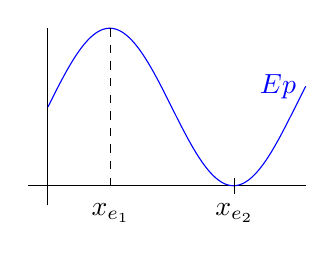
\begin{tikzpicture}
	\draw[] (-0.25, 0) -- (3.28, 0);
	\draw[] (0, -0.25) -- (0, 2);
	\draw[blue, domain=0:3.28, samples=500] plot(\x, {1+ sin(2*\x r)}) node [left] {$Ep$};
	\draw[dashed] (0.8, 2) -- (0.8, -0.1) node [below] {$x_{e_1}$};
	\draw[] (2.37, 0.1) -- (2.37, -0.1) node [below] {$x_{e_2}$};
\end{tikzpicture}

				
\subsubsection{Condition d'équilibre} $\sum_i \vec{F_i} = \vec{0}$ d'après le PFD
\subsubsection{ Position d'équilibre} en $x_e$ :\[\begin{array}{rccl}
				x &=& x_e & \text{ est solution du PFD } \\
		F &=& -\frac{dEp}{dx} = 0\end{array}\]
		Donc $Ep(x)$ est un extremum (avec $x=x_ e$) car la dérivé en $x_e$ est égal à 0.
		\subsubsection{Stabilité de l'équilibre} si on éloigne le système de la position $x_e$, on aura $x = x_e + \Delta x$, avec $\Delta x$ assez petit (négatif ou positif)

Dans ce cas:
\begin{itemize}
	\item Si le système tend à revenir à $x=x_e$, alors la position $x_e$ est une position d'équilibre stable.
	\item Si le système s'écarte de $x=x_e + \Delta$, alors la position $x$ est une position d'équilibre instable.
\end{itemize}

Pour un ressort de raideur $k$, on a:

\begin{center}
	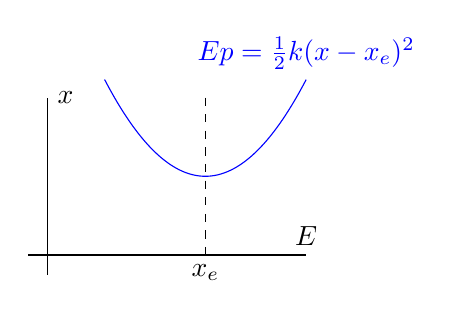
\begin{tikzpicture}
		\draw[] (-0.25, 0) -- (3.28, 0) node [above] {$E$};
		\draw[] (0, -0.25) -- (0, 2) node [right] {$x$};
		\draw[blue, domain=0.72:3.28, samples=300] plot(\x, {1/2 * 1.5 * (\x - 2)*(\x - 2) + 1}) node [above] {$Ep = \frac{1}{2}k(x-x_e)^2$};
		\draw[dashed] (2, 2) -- (2, 0) node [below] {$x_{e}$};
	\end{tikzpicture}
\end{center}

La position d'équilibre stable/ instable est égal au développement limité de $\frac{dEp}{dx}$ à l'ordre 1.
Or en $x=x_e$, $\frac{dEp}{dx} = 0$ par définition de l'équation d'équilibre.

\begin{wrapfigure}[5]{r}{0pt}
	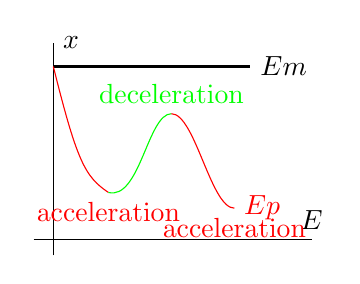
\begin{tikzpicture}
		\draw[] (-0.25, 1) -- (3.28, 1) node [above] {$E$};
		\draw[] (0, 0.8) -- (0, 3.5) node [right] {$x$};
		\draw[thick] (0, 3.2) -- (2.5, 3.2) node [right] {$Em$};
		\draw[red] (0, 3.2) .. controls (0.3, 2) and (0.4, 1.8) .. (0.7, 1.6) node [below] {acceleration};
		\draw[green] (0.7, 1.6) .. controls (1.1, 1.5) and (1.2, 2.6) .. (1.5, 2.6) node [above] {deceleration};
		\draw[red] (1.5, 2.6) .. controls (1.8, 2.6) and (2, 1.4) .. (2.3, 1.4) node [below] {acceleration} node [right] {$Ep$};
	\end{tikzpicture}
\end{wrapfigure}


\[\begin{array}{rcl}
		\text{Donc } \underbrace{\frac{dEp}{dx}}_{x \simeq x_e} &\simeq& \underbrace{\frac{dEp}{dx}}_{x = x_e} + \underbrace{\frac{d^2 Ep}{dx}}_{x = x_e} \cdot  \overbrace{(x-x_e)}^{\Delta x} \\
		\underbrace{\frac{dEp}{dx} }_{x \to x_e} &\simeq& \underbrace{(\frac{(d^2 Ep)}{dx^2})}_{x = x_e} \cdot \overbrace{(x-x_e)}^{\Delta x} \\
		\underbrace{\frac{dEp}{dx} }_{x \to x_e}\cdot \Delta x &\simeq& \underbrace{(\frac{(d^2 Ep)}{dx^2})}_{x = x_e} \cdot (\Delta x)^2  \\
		\underbrace{\frac{dEp}{dx} }_{x \to x_e}\cdot \Delta x > 0 &\Rightarrow& \underbrace{\frac{d^2Ep}{dx^2}}_{x=x_e} > 0 \Rightarrow x_e \text{ est un minimum }
\end{array}\]

\[\begin{array}{rcl}
	Em &=& Ep + \frac{1}{2}m\cdot v^2 \\
	Em \geq 0 && \frac{1}{2}m\cdot v^2 \geq 0 \Rightarrow Ep \geq 0\end{array}\]

Dans un système conservatif donc, la position d'équilibre correspond à un minimum d'$Ep$
\subsection{Système non conservatives}
	L'analyse est la même que dans les systèmes conservatifs, mais il y a un ammortissement dû aux pertes d'énergies (frottements).

	\paragraph{Remarque} Les forces de frottements solides peuvent entrainées des positions d'équilibres mais qui ne sont pas des positions d'équilibres stables.

\chapter{Oscillations}

\section{Introduction} Un ressort, un circuit inductance/condensateur sont des système harmonique oscillateur.

Pour tous ses phénomènes:
\begin{itemize}
	\item Ep est une variable admettant un minimum
	\item la force pour remettre $Ep_{min}$ est linéaire
	\item L'énergie potentielle est quadratique autour de $Ep_{min}$ (elle dépend du carré d'une variable).
\end{itemize}

On obtient dans ces conditions une équation différentielles du type \[\ddot{x} + \omega x = 0\]
La période des oscillations est indépendantes de l'énergie et de l'amplitude du système.

\subsection{Equation du mouvement d'un ressort}
\[\left\{\begin{array}{rcll}
			-kx &=& m\ddot{x}& \\
			\ddot{x} + \frac{k}{m}x &=& 0 \\
			\ddot{x} + \omega^2 x &=& 0 ;\text{ avec } \omega = \sqrt{\frac{k}{m}}
	\end{array}\right.\]


Période propre : $T_0 = \frac{2\pi}{\omega_0}$
Fréquence propre : $\nu_0 = \frac{1}{T_0}$

\subsection{Solution} $x(t) = A\cos (\omega_0 t)+B\sin(\omega_0 t)$.
Avec les conditions initiales, à $t=0, x=x_0$ et $v=v_0$

\[x(t) = x_0\cos(\omega_0 t) + \frac{v_0}{\omega_0}\sin(\omega_0 t)\]

Il est plus facile de représenter $x(t) = X_0 \cos (\omega_0t + \varphi)$

\[\begin{array}{lrclr}
	&x(t) &=& X_0\cos(\omega_0 t + \varphi) \\
	&\dot{x}(t) &=& -\omega_0 \cdot X_0 \sin(\omega_0 t + \varphi) \\
	\text{Pour } t_0 = 0, & x_0 &=& X_0 \cos(\varphi) & (a) \\
	& v_0 &=& -\omega_0 X_0 \sin(\varphi) & (b) \\
	\frac{(b)}{(a)} & \tan \varphi &=& -\frac{v_0}{\omega_0x_0} \\
\end{array}\]

\[\left.\begin{array}{rcl}
	\frac{x_0}{X_0} &=& \cos \varphi \\
	\frac{v_0}{\omega_0 X_0} &=& -\sin \varphi 
\end{array}\right\} \Rightarrow \begin{array}{rcl}
		\frac{x_0^2}{X_0^2} + \frac{v_0^2}{\omega_0^2X_0^2} &=& 1 \\
		X_0 &=& \sqrt{x_0^2 + \frac{v_0^2}{\omega_0^2}} \end{array}\]

\subsection{Notation Complexe}

\[\begin{array}{rcl}
	\ddot{x}+\omega_0^2 x = 0; \text{ solution complexe } \tilde{x}(t) &=& \tilde{A}e^{i\omega_0t} \\
	\tilde{x}(t) &=& Ae^{i\varphi}e^{i\omega_0t} \end{array}\]
Seul la partie réel a un sens physique réel. Cette notation sert à simplifier les calculs.

\[\begin{array}{rclrcl}
	\dot{\tilde{x}}(t) &=& Ae^{i\varphi} (i\omega_0 e^{i\omega_0 t}) &=& (i\omega_0)\tilde{x}(t) \\
	\ddot{\tilde{x}}(t) &=& Ae^{i\varphi} (i\omega_0)^2 e^{i\omega_0 t} &=& (i\omega_0)^2 \tilde{x}(t) \\
	\tilde{x}(t) &=& Ae^{i(\omega_t + \varphi)}\\
	Re(\tilde{x}) &=& A\cos (\omega_0 t + \varphi)
\end{array}\]

\subsection{Aspects énergétique}

\[\left\{\begin{array}{rcl}
	F &=& -kx \\
	  &=& -\frac{dEp}{dx}\end{array}\right. \Rightarrow Ep = \frac{1}{2} k x^2 \]

\[\left\{\begin{array}{rcl}
	x &=& x_0\cos(\omega_0 t) \\
	\dot{x} &=& -\omega_0 x_0 \sin(\omega_0t) \Rightarrow \text{ pour } v_0 = 0 \end{array}\right.\]

\[\begin{array}{rccl}
		Ep (x) &=& \frac{1}{2}k(x_0^2 \cos^2(\omega_0t)) & \omega_0^2 = \frac{k}{m} \\
&=& \frac{1}{2}m\omega_0^2 x_0^2 \cos^2(\omega_0 t) \\
Ec(x) &=& \frac{1}{2}m\dot{x}^2 = \frac{1}{2}m\omega_0^2 x_0^2 \sin^2(\omega_0 t) \\
Em &=& Ec + Ep \\
&=& \frac{1}{2}m\omega^2x_0^2 = constante\end{array}\]

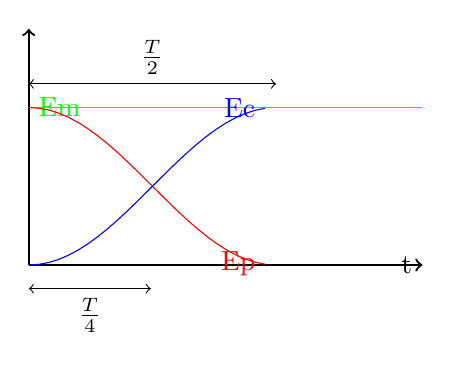
\begin{tikzpicture}
	\draw[->, thick] (0, 0) -- (0, 3);
	\draw[->, thick] (0, 0) -- (5, 0) node [left] {t};
	\draw[green] (5, 2) -- (0, 2) node [right] {Em};
	\draw[red, domain=0:3] plot(\x, {1+cos(\x r)}) node [left] {Ep};
	\draw[blue, domain=0:3] plot(\x, {1-cos(\x r)}) node [left] {Ec};
	\draw[<->] (0, 2.3) -- (3.14, 2.3) node [midway, above] {$\frac{T}{2}$};
	\draw[<->] (0, -0.3) -- (1.55, -0.3) node [midway, below] {$\frac{T}{4}$};
\end{tikzpicture}

\[\text{ a } t=\frac{T}{4}, Ep \text{ se convertie en } Ec\]


